\documentclass{article}
\usepackage[utf8]{inputenc}
\usepackage{graphicx}
\usepackage{subfigure}
\usepackage{amsmath}
\usepackage{color}
\title{SleepWell}
\author{Hackthoner}
\date{December 2021}
\newtheorem{assump}{Assumption}
\usepackage{cite}
\usepackage{appendix}
\begin{document}

\maketitle

\begin{abstract}
As the COVID-19 pandemic spreads across the globe, school systems have been shutting their doors in many countries and a large number of children have been out-of-school. Therefore, we are again reminded of the catastrophic education emergency worldwide lockdown have created and the urgency of achieving Quality Education (SDG 4) goal by 2030. The education community has indeed done a lot of work, including exploring the relation between the pandemic and school closures, as well as different control measures, such as using e-learning tools to continue education activities. However, there has been little discussion about how participation of children in educational activities affected by their access to remote learning tools under school closures caused by COVID-19. In an attempt to better understand the quantitative effect, the data of 13 Latin American countries were chosen to utilize statistical tools such as change point detection and generalized linear model. The result showed that remote learning services can greatly benefit learning for out-of-school children to continue education activities during the pandemic. The fitted model was also used to predict the percentage of access to any education activity of other countries. Our work reveals the significance of strengthening the resilience of the education system by allocating appropriate and adequate resources before a crisis.
\end{abstract}

\section{Introduction}
\label{Introduction}
How COVID-related learning loss benefit from access to remote learning services.


The COVID-19 pandemic has caused the largest disruption of education systems in history, affecting nearly 1.6 billion learners in more than 190 countries and all regions, and more than 168 million children have been reported completely out of school due to school closure policies \cite{Closure168}. Though such impact varies from country to country, the fact is that poor and developing countries remain the most fragile. For developing countries and poor regions, the pandemic has stretched their very limited educational resources even further. Most children from developed countries have access to high-quality online learning facilities at home to continue education activities during the pandemic, while many students from poor countries even lack textbooks and other educational resources before the pandemic\cite{AZUBUIKE2021100022}. For some countries from Latin America and the Caribbean (LAC) Region, the governments were even not able to replenish necessary learning resources, not to mention to provide all students in public schools with the tools they need to learn online.  

In addition, even though governments and relevant Non-Governmental Organizations (NGOs) have the ability to provide these students with laptops, smartphones or tablets, Internet connectivity which depends on the country’s telecommunications infrastructure and power station for electricity\cite{OnlinenRemote} are also needed. 

Therefore, this study aims to explore how the severity of COVID-19 pandemic, school closures, online education access(measured by electricity, Internet, etc.) affect the access to education. We follow a intuitively convincing logic:

\begin{itemize}
    \item \textbf{COVID 19 leads to school closure.} This statement is supported by hypothesis testing\ref{test} and change point detection \ref{change} method. The analysis provides quantitative evaluation on policy and pandemic development.
    \item \textbf{Access to education partitions into access to school and access to remote learning.} Variables in both category are used to predict access to education and develop a framework of approximation. 
\end{itemize}

From a SDG 4 perspective, we argue that our statistical models serve as counselor for countries and government to facilitate policy making. Numeric results help to make a more precise decision, and thus promote educational development. At 2030, we do not only hope to achieve SDG 4 goals, but also want a efficient information collection system that minimize the trade-off between cost and accuracy. Such approximation framework will indeed be necessary part of such system. 


The paper is organized as follows. Section \ref{Introduction} presents the background, motivation and objectives of our study. Methodologies including T test, change point detection and regression models are in Section \ref{Methodology}. Data sources, processing and descriptive analysis are in Section \ref{DataExploration}. Section \ref{closure} quantitatively evaluate the relationship between school closure and pandemic. Section \ref{prediction} provides approximation framework for access to education data under pandemic. 

\section{Methodology}
\label{Methodology}
\subsection{T Test}
\label{test}

We give a brief introduction to student T test on Wiki \cite{Ttest}.
"The t-test is any statistical hypothesis test in which the test statistic follows a Student's t-distribution under the null hypothesis.A t-test is the most commonly applied when the test statistic would follow a normal distribution if the value of a scaling term in the test statistic were known. When the scaling term is unknown and is replaced by an estimate based on the data, the test statistics (under certain conditions) follow a Student's t distribution. The t-test can be used, for example, to determine if the means of two sets of data are significantly different from each other."
\subsection{Change Point Detection}
\label{change}
It's natural to consider algorithm in time series analysis since data sets appear mainly in form of time series or so called panel data. Time series data are sequences of observations over time describing the behavior of systems. These behaviors can change over time due to external events or internal systematic changes in dynamics/distribution . Change point detection (CPD) is the problem of finding abrupt changes in data when a property of the time series changes \cite{CPD1}. 
Partition, anomaly detection, event detection, and edge detection are similar concepts, all of which are occasionally applied as well as change point detection. Change point detection is closely related to the well-known problem of change point estimation or change point mining \cite{CPD2}. 

We from here on introduce methodology side of change point detection, with a special attention on off-line detection since our data do not possess high frequency and main principal aspect of this project do not involve prediction.

Several basic definitions are required in convenience of following introduction. We define a \textit{time series data} an infinite sequence of elements 

\begin{equation}
S=\left\{x_{1}, \ldots, x_{i}, \ldots\right\}
\end{equation}

where $x_i$ is d-dimensional data vector with time i. A time series is \textit{stationary} if 1) $E x_t$ is invariant 2) $cov(x_s,x_t)=E (x_s-E x_s) (x_t-E x_t)$ depends only on $|s-t|$. Given stationary time series S and S' of length T and T', with different potential distribution. Define a \textit{change} point T if T segment two stationary time series.For in stance, T is a change point of time series $\{S,S'\}$ since distribution before and afterwards T has changed. 

General change point detection algorithm take the following form of cost function 
$$
V(\mathcal{T}, x):=\sum_{k=0}^{K} c\left(x_{t_{k} \cdot t_{k+1}}\right)
$$
where $\mathcal{T}$ is a segmentation of time series $X$. $c(\cdot)$ is a cost function which measures goodness-of-fit of the sub-signal $
x_{t_{k} \cdot t_{k+1}}=\left\{x_{t}\right\}_{t_{k}+1}^{t_{k+1}}$. For instance, let
$$
c(x_1^{t})=\sum_{i=1}^{t}(x_i-\Bar{x})^2
$$
where $\Bar{x}$ is mean of xs. This $l_2$ penalty push sample from each segmentation to be close in $l2$ sense. The best segmentation is the minimizer of $V(\mathcal{T},x)$. 

Basing on domain knowledge we have access to, change point detections fall into two type:

\begin{itemize}
    \item Known number of changes. Then we focus on 
$$
\min _{|\mathcal{T}|=K} V(\mathcal{T})
$$
 meaning that finding minimizer in segmentation with K segment points.
 \item Unknown number of changes. Then we focus on $$
\min _{\mathcal{T}} V(\mathcal{T})+\operatorname{pen}(\mathcal{T})
$$ where $pen(\mathcal{T})$ is an appropriate measure of the complexity
of a segmentation. It takes common form of "cost and penalty" wildly adopted in machine learning community. 
\end{itemize}

We focus on the second case. Common penalties such as  $l_0$\cite{10.1214/09-SS054}($\beta|\mathcal{T}|$)  $BIC$\cite{YAO1988181}($\frac{p}{2}logT|\mathcal{T}|$, p is dimension of parameter space) can be directly adopted, with mild assumption on potential distribution. Other method such as mBIC\cite{LEBARBIER2005717}, $l_1$\cite{Hocking2013} and AIC\cite{doi:10.1198/jasa.2010.tm09181} can also be considered under certain assumptions of potential distribution. 

Searching method takes up another part of methodology topology of change point detection. Available instance are Pelt \cite{doi:10.1080/01621459.2012.737745}, a optimal method for unknown number of changes, and other approximate detection such as window sliding \cite{10.1214/08-AOAS232} and binary segmentation \cite{Sen197598}. 

Ruptures\cite{Ruptures} is a Python library for off-line change point detection. This package provides methods for the analysis and segmentation of non-stationary signals.

\subsection{Regression Models}

Regression has attracted immense interest lately due to its effectiveness in tasks like predicting values. And Regression is of widespread use in multiple fields such as Economics, Finance, Business, Biology and so on. 

Regression is an approach of obtaining a relationship between input space and output space. Data takes form of  $\left\{(x_1,y_1),(x_2,y_2),...,(x_n,y_n)\right\}$, which $y_i  \in R$. We intend to train a model from our data set and implement it in unknown test sets to achieve low residue $\epsilon$
% \begin{equation}
\begin{subequations}
\renewcommand{\theequation}{\theparentequation.\arabic{equation}}
\begin{align}
y &= \hat{y} + \epsilon \\
  &= f(x) + \epsilon 
\end{align}
\end{subequations}

% \end{equation}


Ordinary Least Squares takes the form where $f(x)=\theta x$.
To improve the generality of the model, useful loss functions are created. The objective function of ridge is composed of the usual regression loss (i.e. Mean Squared Errors) and L-2 penalty \cite{ridge}. 
\begin{equation}
        J(\theta) = \frac{1}{n}\sum \limits_{i} ^ {n} (y_i -                    \hat{y_i})^2 + \frac{\lambda}{2}||\theta _i||^2          
  \end{equation}

Logistic regression, one of the simplest yet powerful generalized linear model, is suitable when y vary in 0 to 1. It takes the following form
$$
\ell=\log _{b} \frac{p}{1-p}=\beta_{0}+\beta_{1} x_{1}+\beta_{2} x_{2}
$$



\section{Data Exploration}
\label{DataExploration}
\subsection{Data Set Description}
 
\begin{itemize}


\item Cases and deaths of COVID-19 data set. Data set consists of daily statistics of new cases and new deaths in 239 countries from Jan 3, 2020 till up to date.

\item School closure data set. Data set consists of items of daily status of schools from 210 countries, ranging from Feb 16, 2020 to Oct 31, 2021. Schools may possess one of the four status: fully open, partially open, closed due to COVID-19 and academic break. 

\item Access to remote learning for students data set. This data set contains information about the access to remote learning tools by students, which contains 18 variable of 20 countries. It is maintained by \cite{maintained}. We manually add data of the access to electricity, mobile, and internet in 13 LAC countries from \cite{WorldBank}. 

\item Access to education data set. This data set contains data of 13 countries, Bolivia, Chile, Colombia, Costa Rica, Dominnican Repubilc, Ecuador, El Salvador, Guatemala, Honduras, Mexico, Paraguay, Peru, Saint Lucia, all of which belong to Latin America \& the Caribbean. Data is percentage of children have NOT been engaged in any education or learning activities since the schools closed. 


\end{itemize}

\subsection{Data Set Processing}

\begin{itemize}

\item Referring to World Bank Regional Units, we focused on the countries in these six units in following studies(see Table1). The total amount of the countries is 141.


\begin{table}[]
\setlength{\belowcaptionskip}{0.2cm}
\label{Tab:1}
\caption{World Bank Regional Units and the amount of countries}
\centering
\begin{tabular}{lcc}
\hline
Regional Units                 & Code & Number of Countries    \\ \hline
Africa                         & SSA & 48    \\ 
East Asia \& Pacific           & EAP & 14    \\
Europe \& Central Asia         & ECA & 23    \\
Latin America \& the Caribbean & LAC & 30    \\
Middle East \& North Africa    & MNA & 18    \\
South Asia                     & SAR & 8    \\ 
Total                          &     & 141  \\ \hline
\end{tabular}
\end{table}

\item School closure data set. Data set is transformed into panel data with each row being a panel of concurrent daily status in different countries. Country names in-consistency with other data set, due to different convention of data source, is unified for each entity. Data set is constrained to 141 countries mentioned before.

\item Cases and deaths of COVID-19 data set. Data is transformed into panel data with each row being a panel of concurrent daily status in different countries. Note that data set contains negative increase cases and possess characteristic of great volatility. Negative values may attribute to measurement error and statistical organization may add correction to following day's data. We conquer this by averaging successive 7 day's increase numbers of every time channel. Sight behind that allows us to do so is the common assumption of continuity or even smoothness of COVID-19 increase curve \cite{SHUR21,Alvarez21}. As in general setting in infectious diseases modeling, only mild condition is required such as SIR model \cite{kermack}
$$
\frac{d i}{d t}=b s(t) i(t)-k i(t)
$$
where i stands for infected population.
And Since we aim to analyze the difference between different regions, the data set is combined daily for each region.



\end{itemize}

\subsection{Summary Statistics}
\begin{itemize}
\item \textbf{LAC region has suffered a lot during the pandemic}. Figure \ref{fig:covid-19} shows that all regions shared a similar increasing trend of daily new cases and deaths between March and August 2020, and LAC is obviously the region which mostly affected by the COVID-19 pandemic. Its daily reported new cases and deaths even reached 107,325 and 4,277 respectively in July. 
\begin{figure}[ht!]
\centering
 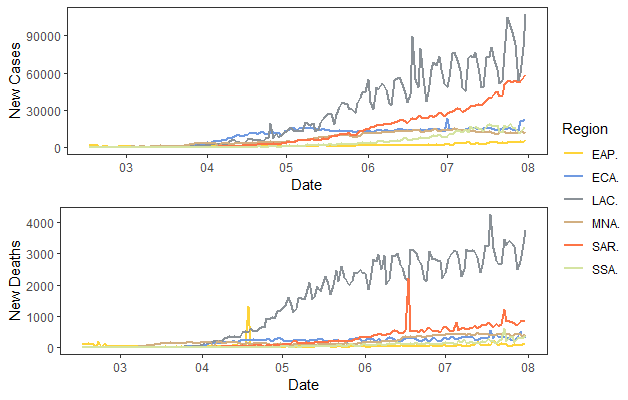
\includegraphics[width=0.9\textwidth]{covid.png}
\caption{Daily New Cases and Deaths due to COVID-19 from February 2020 to December 2021}.
\label{fig:covid-19}
\end{figure}

\begin{table}[]
\setlength{\belowcaptionskip}{0.2cm}
\label{Tab:2}
\caption{Duration of School closure in Weeks of Each Region from February 2020 to December 2021}
\centering
\begin{tabular}{lllllll}
\hline
Regional Units                 & Code & Mean±Se   \\ \hline
Africa                         & SSA & 16.79±0.74    \\ 
East Asia \& Pacific           & EAP & 15.00±1.39    \\
Europe \& Central Asia         & ECA & 10.95±1.07    \\
Latin America \& the Caribbean & LAC & 18.57±0.78    \\
Middle East \& North Africa    & MNA & 14.33±0.93    \\
South Asia                     & SAR & 21.12±1.31    \\  \hline
\end{tabular}
\label{Tab:school_closed}
\end{table}

\item \textbf{Numerous countries closed schools during the pandemic}. With the COVID-19 outbreak and spreading across the globe, schools have been completely or partially closed due to national COVID-19 lockdown. LAC is one of the regions which holds the number of countries that closed schools due to COVID-19, and SSA is the other(\ref{fig:school_closed}). What's more, Table \ref{Tab:school_closed} also showed that SAR and LAC regions had kept schools closed for the most weeks between March and August 2020 (21 weeks and 18 weeks, respectively), followed by SSA, EAP, MNA and ECA region.

\begin{figure}[ht!]
\centering
 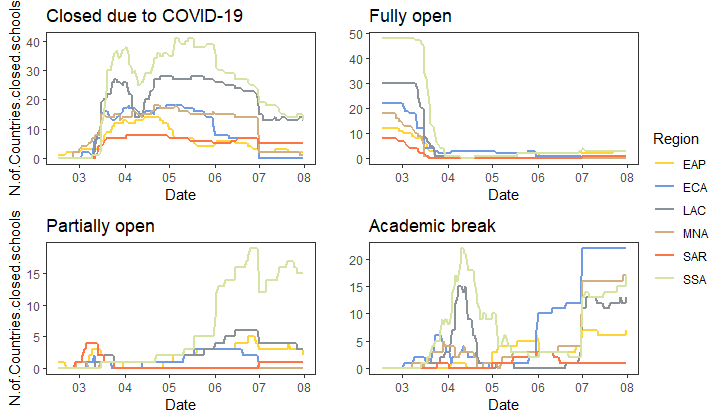
\includegraphics[width=0.9\textwidth]{school_closed.png}
\caption{Numbers of Countries Closed Schools during the Pandemic of Six Regions from February 2020 to December 2021}.
\label{fig:school_closed}
\end{figure}

\item \textbf{The percentage of children with e-learning services at home in some regions is relatively low}. Figure \ref{fig:remote_learning} presents that with schools closed during the pandemic, many countries broadcast lessons over TV or radio channel to keep children learning. All regions report high percentage (over 95\%) of children have access to electricity and mobile at home except SSA (47.85\%, 78.27\%). However, the percentage of children’s access to radio, television, computer and internet varies greatly from region to region.

\begin{figure}[ht!]
\centering
 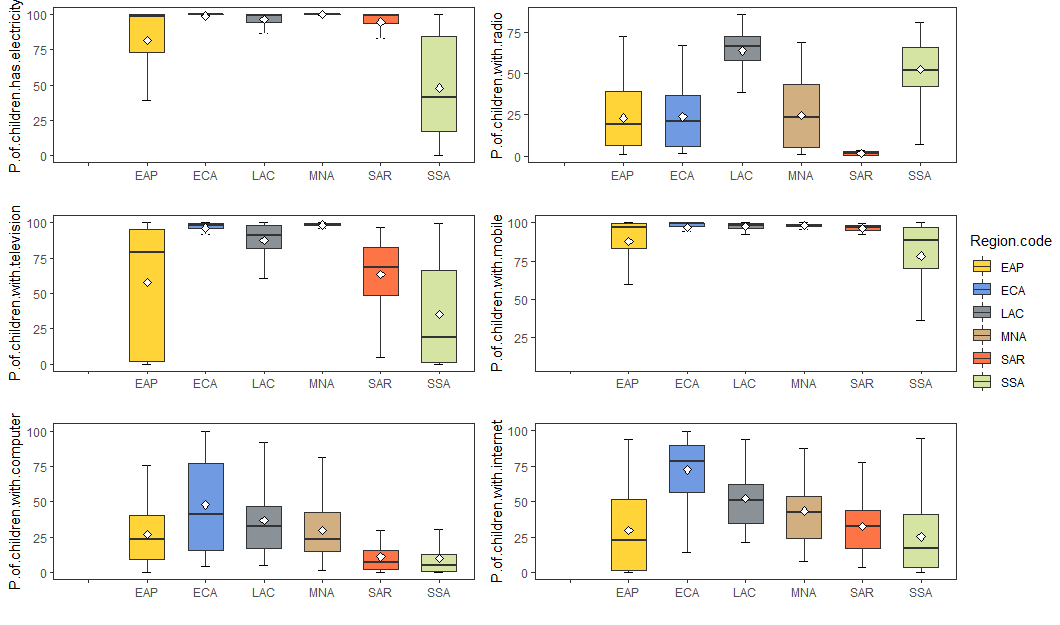
\includegraphics[width=0.9\textwidth]{remote_learning.png}
\caption{Access to Remote Learning Services of Six Regions}.
\label{fig:remote_learning}
\end{figure}

\item \textbf{Most children have not been engaged in any education or learning activities since school closed in LAC region}. Table 3. reports the percentage of children who have not been engaged in any education or learning activities since school closed in LAC region. We can find that countries such as Bolivia and Guatemala and St.Lucia report nearly 10\% of school age children not engaging in any education activity. It is long till we will see achievement of SDG.

\begin{table}[]
\setlength{\belowcaptionskip}{0.2cm}
\label{Tab:2}
\caption{Percentage of Non-Access to Education of 13 Countries in LAC Region}
\centering
\begin{tabular}{ccccccccc}
\hline
Country      & Percentage of Non-Access to Education\\ \hline
Bolivia          & 15.2\%    \\ 
Chile          & 4.1\%    \\
Colombia          & 3.3\%    \\
Costa Rica          & 3.1\%    \\
Dominican Republic          & 6.1\%    \\
Ecuador          & 2.6\%    \\
El Salvador          & 1.9\%    \\
Guatemala          & 9.8\%    \\
Honduras          & 7.8\%    \\
Mexico          & 2.1\%    \\
Paraguay          & 1.4\%    \\
Peru          & 2.8\%    \\
St. Lucia          & 8.5\%    \\  \hline
\end{tabular}
\end{table}

\end{itemize}


\section{School Closure and Pandemic Severity}
\label{closure}
To fulfill the purpose of our study, we seek to better understand how the implementation of public health policy (in our case, school closure policy) measures at a national scale is reflected in the actual trend of the daily new cases in each corresponding country. Our data analysis approach consists of two parts. The first is to draw summary statistics from corresponding policy period to see statistical relationship between. From a hypothesis testing perspective, the correlation is well presented. We also hope to find, to some extent, interact dynamic between policy and progress of pandemic. It suffice to show potential and subtle changes in pandemic trend coincide with national policy for each country. This question can be answered by using statistical change point models, which is the second part of our analysis. The identified change points combined with the school closure time line can provide interpretation of how they interact. \cite{COUGHLIN2021100064} considered this method dealing with pandemic data from 20 countries and first recorded shut down policies. Their results are satisfying with intuitively correct result and detailed logical analysis. Relationship between K-12 school opening and spread of COVID-19 is also considered \cite{Chernozhukove2103420118}. We note that the paper also include a elementary discussion of association between school openings and mobility. They provides a two fold conclusion: 1) Opening K–12 schools increases the number of contacts within schools. 2) Reopening K–12 schools allows parents to return to work and increase their mobility in general, which may contribute to the transmission of COVID-19 at schools and workplaces. This conclusion seems to be an antinomy. But telescoping analysis is still feasible with available data in public and school visits. Due to data limitation, we conduct elementary analysis in school closure and the pandemic. 
We first make a simple assumption of data.
\begin{assump}
We assume that status given in the data represents ground truth of school closure i.e. we ignore minority of schools inconsistent with reported status. 
\end{assump}


\subsection{Hypothesis Testing}
Summary statistics based on COVID-19 cases and deaths is shown in Table \ref{Tab:cases2}. Averaged daily observations is reported with respect to school status in form of mean and variance. We consider three countries, China, Japan and US, as representatives of other countries in the world. We also report difference in mean with status of fully open and other status. As auxiliary information, we conduct two sample T-test of observations with status of fully open and other status and present whether inferential statistic is below significant level of 0.05. This roughly justify whether they are identically distributed, serving as evidence of our argument about correlation between school closure and severity of pandemic. We pay specially attention to data in United States. Since status "Partially open" and "Academic break" take up majority of data reported from US, we compare status "Partially open" with "Academic break". From the results we can see, China experience a first emerge of COVID-19 during winter break and a drastic growth afterwards with school shut down. But with mighty lock down policy, situation is soon under control and reopening of school. Thus school closed period has higher increase. This "all-cleaning" strategy results in difference behavior of new cases data comparing to so called "coexist" strategy. Under such strategy, increasing never stops and reduce when school shut down (usually with company of other control policy), which appears in Japan and US case. Conclusions we draw are two-fold:

\begin{itemize}
    \item \textbf{School closure and severity of pandemic are highly correlated.}
    \item \textbf{Relationship between should be considered country-wise. }
\end{itemize}

A special telescoping on LAC countries is displayed in Table \ref{Tab:cases2}. Averaged daily observations is reported with respect to school status in form of mean and variance. Here we consider countries from LAC, Chile, Colombia, Mexico and Peru as representatives of other countries in the continent. Similar process of changing testing category is down for highly imbalanced reported data. Still, a similar statement can be made inside Latin America. 


\begin{table}[ht]
\centering

\caption{
Summary statistics based on COVID-19 cases and deaths observations from February 2020 to December 2021.  }

\begin{tabular}{ccccccccc}
\hline
       & \multicolumn{2}{c}{Fully} & \multicolumn{2}{c}{Partially} & \multicolumn{2}{c}{Closed} & \multicolumn{2}{c}{Break} \\ \hline
\multicolumn{9}{c}{China}                                                                                                                      \\ \hline
       & Mean          & Var       & Mean           & Var          & Mean       & Var      & Mean           & Var          \\ \hline
Cases  & 98.5          & 127.2          & 83.8           & 340.3             & 146.4      & 187.4         & 75.2           & 51.9              \\
Deaths & 2.8           & 6.5            & 4.9            & 22.9              & 36.4       & 158.8         & 1.4            & 1.7               \\ \hline
       & Diff          & Sign.          & Diff           & Sign.       & Diff       & Sign.   & Diff           & Sign.       \\ \hline
Cases  &               &                & 14.6           & False             & 47.9       & True          & -23.2          & True              \\
Deaths &               &                & 2.1            & False             & 33.6       & True          & -1.5           & True              \\ \hline
\multicolumn{9}{c}{United States}                                                                                                              \\ \hline
       & Mean          & Var       & Mean           & Var          & Mean       & Var      & Mean           & Var          \\ \hline
Cases  & 2.5           & 2.2            & 76149        & 62642           &            &               & 69588        & 56339           \\
Deaths &               &                & 1343.4         & 907.0             &            &               & 803.7          & 672.2             \\ \hline
       & Diff          & Sign.          & Diff           & Sign.       & Diff       & Sign.   & Diff           & Sign.       \\ \hline
Cases  &               &                &         &               &            &               & -6561.0        & True              \\
Deaths &               &                &          &               &            &               & -539.7          & True              \\ \hline
\multicolumn{9}{c}{Japan}                                                                                                                      \\ \hline
       & Mean          & Var       & Mean           & Var          & Mean       & Var      & Mean           & Var          \\ \hline
Cases  & 2216.9        & 2683           & 242.5          & 202.3             & 39.8       & 14.8          & 7288.2         & 7918.0            \\
Deaths & 34.5          & 33.7           & 14.7           & 13.4              & 1.54       & 1.84          & 20.6           & 17.7              \\ \hline
       & Diff          & Sign.          & Diff           & Sign.       & Diff       & Sign.   & Diff           & Sign.       \\ \hline
Cases  &               &                & -1974.4        & True              & -2177.1    & True          & 5071.3         & True              \\
Deaths &               &                & -19.8          & True              & -33.0      & True          & -13.9          & True              \\ \hline
\end{tabular}
\\

\label{Tab:cases1}
\end{table}



\begin{table}[]
\caption{Summary statistics based on COVID-19 cases and deaths observations of from February 2020 to December 2021. }
\begin{tabular}{ccccccccc}

\hline
       & \multicolumn{2}{c}{Fully open} & \multicolumn{2}{c}{Partially open} & \multicolumn{2}{c}{Closed} & \multicolumn{2}{c}{Academic break} \\ \hline
\multicolumn{9}{c}{Chile}                                                                                                                      \\ \hline
       & Mean         & Var        & Mean           & Var          & Mean      & Var       & Mean           & Var          \\ \hline
Cases  & 2.1          & 4.1             & 2834.4         & 2276.7            & 2853.2    & 4034.5         & 2889.0         & 1378.8            \\
Deaths &              &                 & 65.0           & 68.2              & 57.7      & 95.4           & 62.3           & 43.8              \\ \hline
       & Diff         & Sign.           & Diff           & Sign.       & Diff      & Sign.    & Diff           & Sign.       \\ \hline
Cases  &              &                 & 2832           & True             & 2851      & True           & 2886.9         & True              \\
Deaths &              &                 & 65.0           & True             & 57.7      & True           & 62.2           & True            \\ \hline
\multicolumn{9}{c}{Colombia}                                                                                                                   \\ \hline
       & Mean         & Var        & Mean           & Var          & Mean      & Var       & Mean           & Var          \\ \hline
Cases  & 1.0          & 2.3             & 10081.4        & 8147.2            & 4342.6    & 4040.9         & 9088.2         & 6359.0            \\
Deaths &              &                 & 252.8          & 184.0             & 139.0     & 125.1          & 188.5          & 131.0             \\ \hline
       & Diff         & Sign.           & Diff           & Sign.       & Diff      & Sign.    & Diff           & Sign.       \\ \hline
Cases  &              &                 & 10080          & True              & 4341.6    & True           & 0              & True              \\
Deaths &              &                 & 252.9          & True              & 139.0     & True           & 188.6          & True              \\ \hline
\multicolumn{9}{c}{Mexico}                                                                                                                     \\ \hline
       & Mean         & Var        & Mean           & Var          & Mean      & Var       & Mean           & Var          \\ \hline
Cases  & 25.1         & 40.9            & 5914.2         & 3791.4            & 5314.5    & 14.8           & 7288.2         & 7918.0            \\
Deaths & 0.1          & 0.5             & 303.5          & 197.2             & 515.5     & 1.84           & 20.6           & 17.7              \\ \hline
       & Diff         & Sign.           & Diff           & Sign.       & Diff      & Sign.    & Diff           & Sign.       \\ \hline
Cases  &              &                 & 5889.1         & True              & 5289.4    & True           & 10674.7        & True              \\
Deaths &              &                 & 303.4          & True              & 515.4     & True           & 581.4          & True              \\ \hline
\multicolumn{9}{c}{Peru}                                                                                                                       \\ \hline
       & Mean         & Var        & Mean           & Var          & Mean      & Var       & Mean           & Var          \\ \hline
Cases  & 1.6          & 3.5             & 2819.5         & 2293.0            & 4074.6    & 2883.9         & 4986.1         & 2377.5            \\
Deaths & 0.1          & 0.3             & 197.9          & 196.1             & 425.2     & 255.7          & 471.2          & 230.7             \\ \hline
       & Diff         & Sign.           & Diff           & Sign.       & Diff      & Sign.    & Diff           & Sign.       \\ \hline
Cases  &              &                 & 2817.9         & True              & 4073.0    & True           & 4984.5         & True              \\
Deaths &              &                 & 197.8          & True              & 425.1     & True           & 471.1          & True              \\ \hline
\end{tabular}

\label{Tab:cases2}
\end{table}



\subsection{Change Point Detection}
As explained in Section \ref{Methodology}, change point detection attempts to identify the time when the probability distribution of a random process or time series changes. Generally speaking, the question involves detecting whether a change has occurred, or whether several changes may have occurred, and the time to identify any such changes. We use package \cite{Ruptures} for detection. We follow a convention of toy experiment, setting searching method to binary segmentation and penalty form to $l_2$ loss. Illustrating results are presented in Fig \ref{fig:changepoint1}. 




    \begin{figure}[ht!]
\centering

    \begin{subfigure}{\textwidth}
    	\centering
        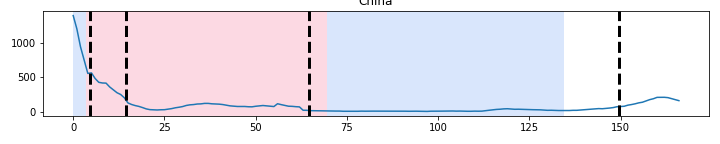
\includegraphics[width=0.9\textwidth]{_China.png}
    \end{subfigure}
    \begin{subfigure}{\textwidth}
    	\centering
        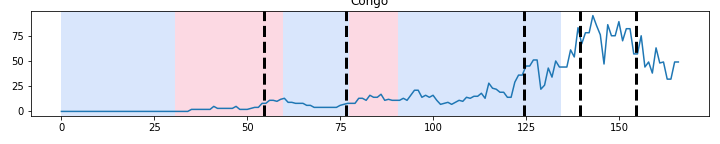
\includegraphics[width=0.9\textwidth]{_Congo.png}
    \end{subfigure}
  
    \caption{Plot of change point detection and school status. Data utilized to perform change point detection is new cases of COVID 19 data from Feb 14 2020 to July 31 2020 in one country, being consistent with analysis and downstream task. Background color stands for alternate of school status in corresponding country, which we categorize into "open", with original status "Fully open" and "Partially open", and "closed", with original status "Closed" and "Academic break". Toy illustration of China and Congo is presented for analysis convenience. Exhaustive result is in Fig \ref{fig:changepoint2}. }.
\label{fig:changepoint1}
\end{figure}

We now analysis the result. Cases curves are quite different in each country, so it's apparent that we take country-wise analysis. As in the case of China, four change points are identified. First two intuitively corresponding to control of COVID 19 in first half of 2020. Schools reopen as soon as epidemic is under control. We, as witnesses of this stage victory, interpret school reopening as consequence of control of pandemic. As in case of Congo, change points identified are located around changing status of school. These two vanilla model example provides evidence in interaction between pandemic trend and national policy within country. More cases are displayed in Fig \ref{fig:changepoint2}.

\section{Predictions made by Regression}
\label{prediction}
To further explore the relationship between the independent and dependent variables, we choose the regression models. In order to make the regression task theoretically legal, we make an assumption first.
\begin{assump}
We assume distribution of access to education (AE) since school closed due to pandemic conditioning on access to remote learning (RL) variables, severity of COVID 19 (CO) and school policy (SP) is approximately identical for every country. 
$$
P( \text{AE}|\text{country})\approx P(\text{AE}| \text{RL}, \text{CO}, \text{SP})
$$
Reason that this is capable is the explanation in the survey. "In each of these cases, the two most reported reasons were lack of availability of internet and teacher-related problems (e.g. no contact with pupils or no provision of homework)." Thus, information contained in the three parts combine to explain access to education. 
\end{assump}


For regression data we use, note that independent variables are the duration of full and partial school closures in weeks, new cases of COVID-19, the percentage of children who have electricity at home, the percentage of children with mobile at home and the percentage of children with internet at home. The dependent variable is the non-access to education. And all countries are in Latin America and the Caribbean.

\begin{figure}[h]
\centering
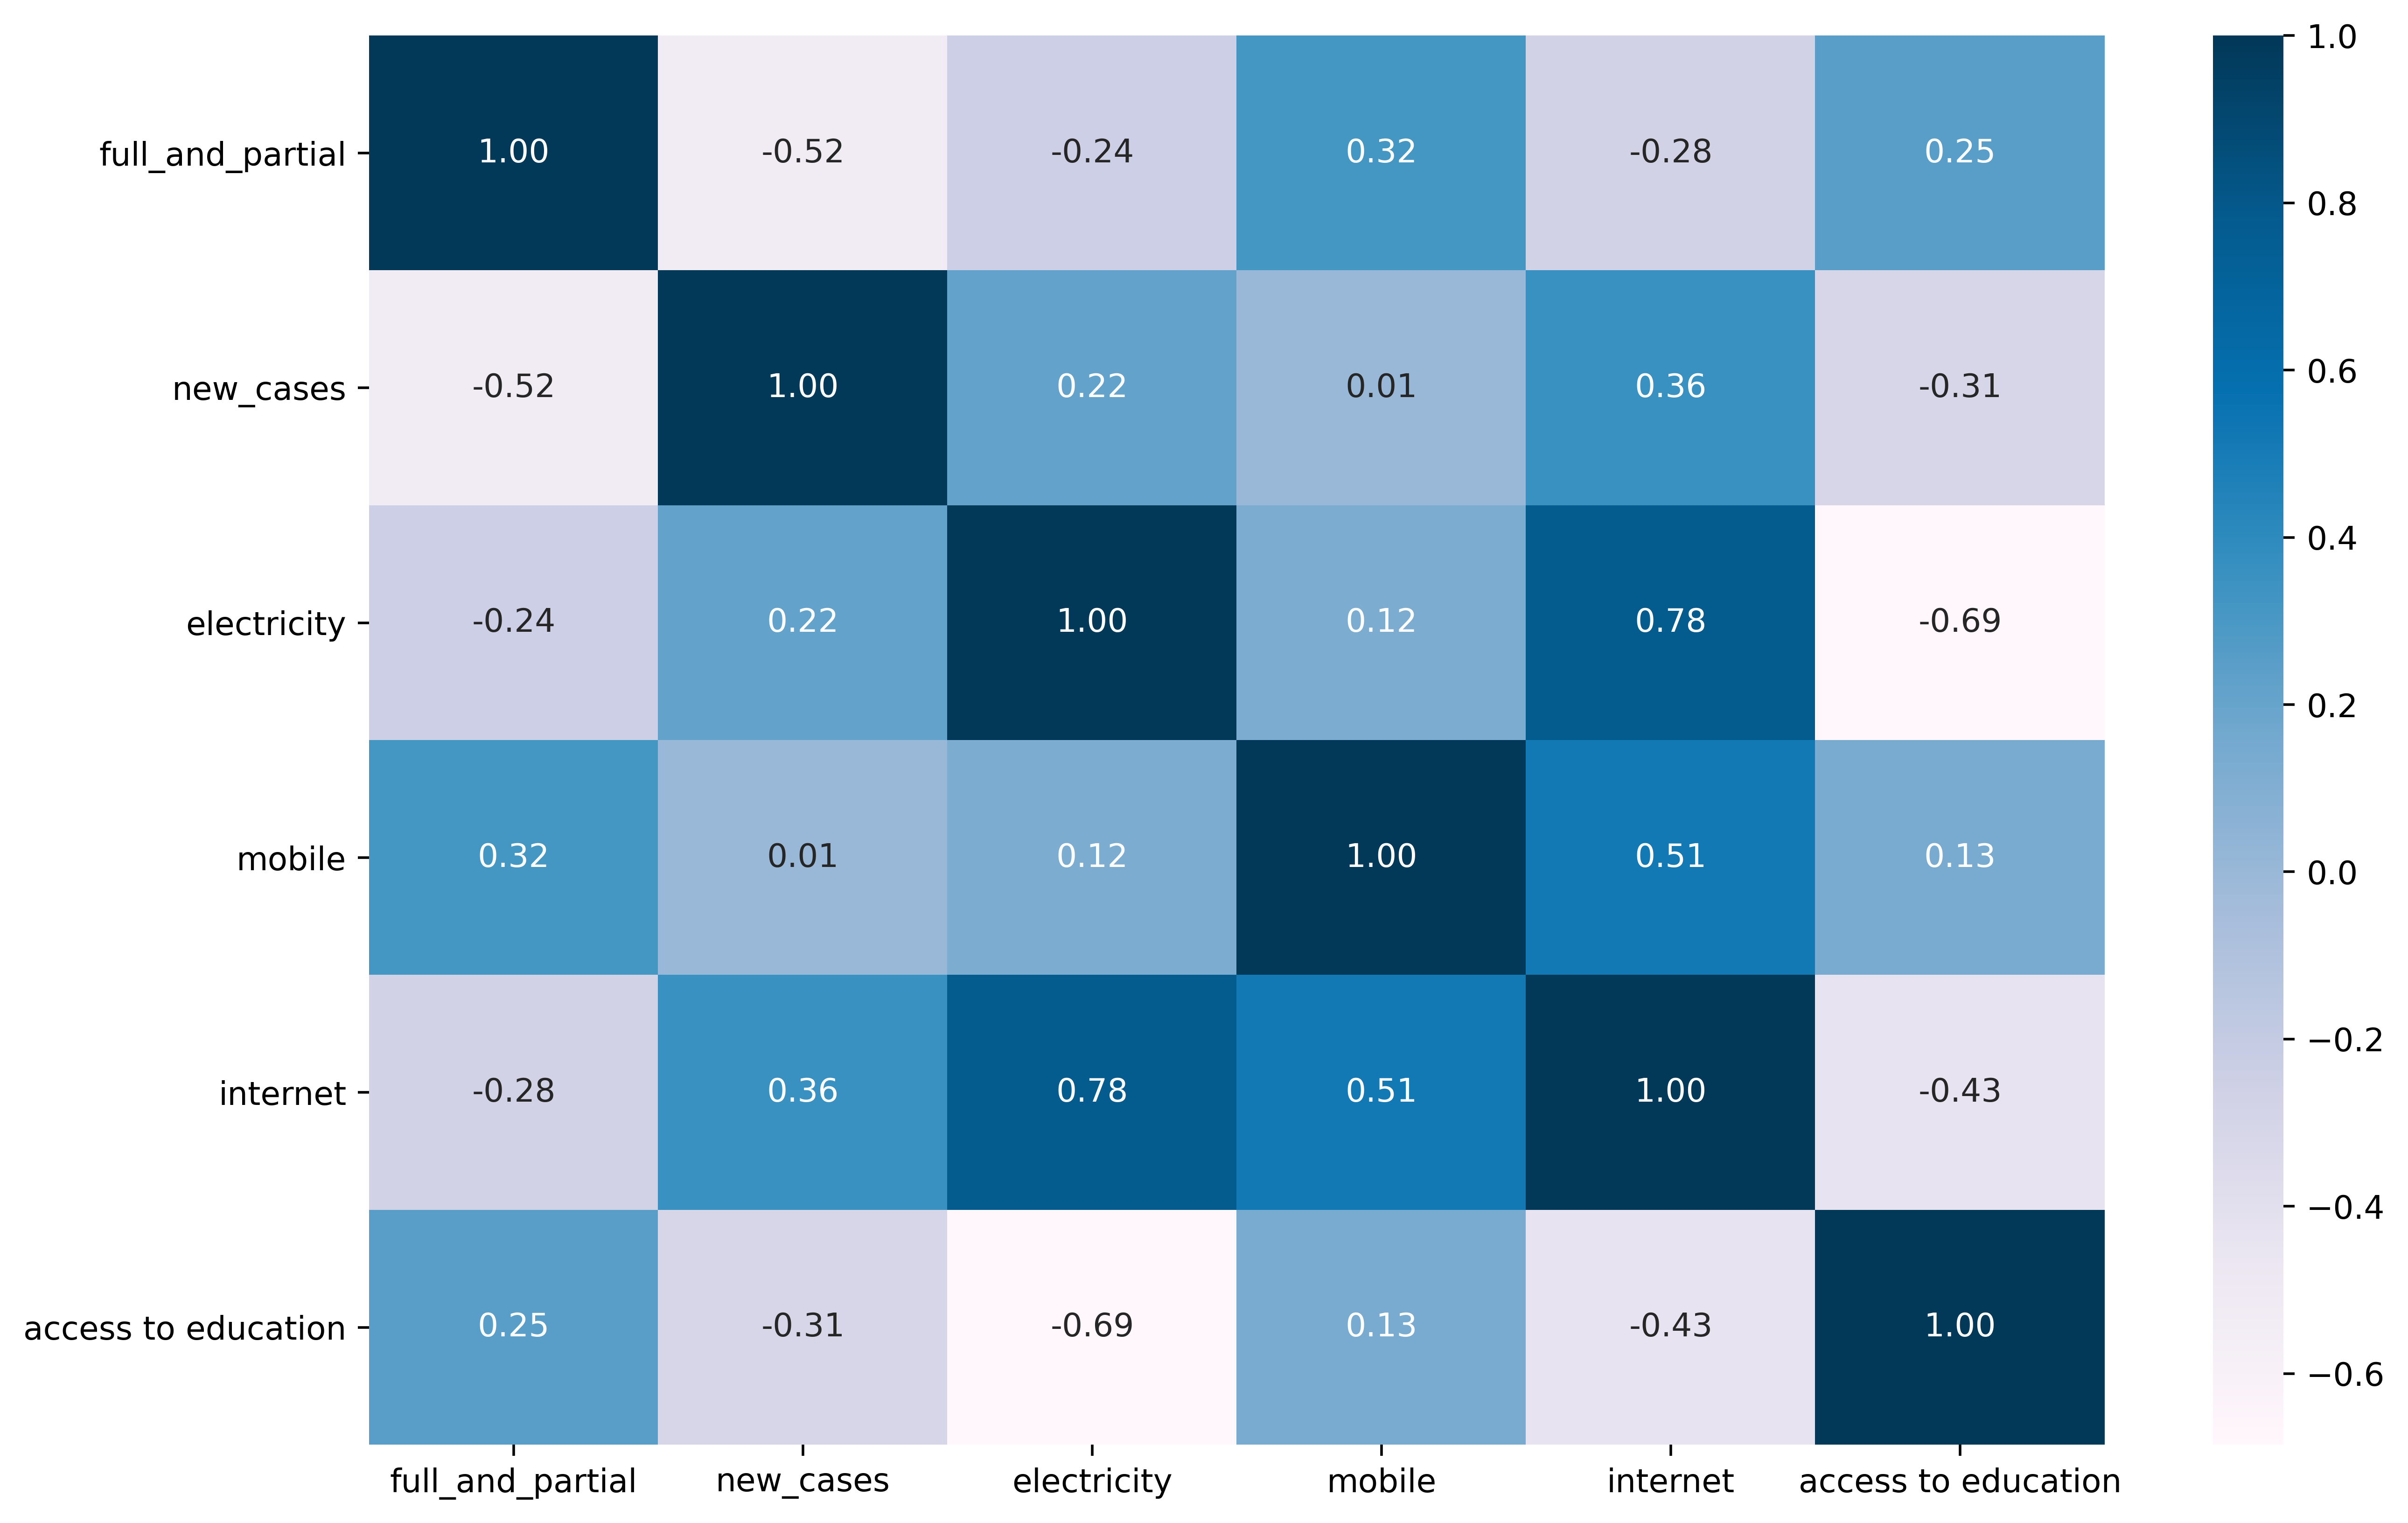
\includegraphics[width=1.0\columnwidth]{heatmap.png}% Reduce the figure size so that it is slightly narrower than the column. Don't use precise values for figure width.This setup will avoid overfull boxes. 
\caption{This shows the relationship between the independent and dependent variables in the heatmap.}
\label{fig3}
\end{figure}

As observed in the heat map Fig \ref{fig3}, the relationships between them can be interesting and valid. For instance, the percentage of children with internet at home is in positive correlation with the percentage of children who have electricity at home and in negative correlation with the duration of full and partial school closures in weeks. Because the heat map can only show pairwise relationship, we continue to use specific regression models to model the variables. The output coefficients below is predicted by ridge regression.
\begin{equation}
    \rm Coefficient = [0.619, 1.833, -1.742, 1.235, -0.638]
\end{equation}

The result demonstrate that new cases is in the strongest positive correlation with non-access to education, which further confirms correlation between the severity of COVID-19 and the access to education suggested by many news reports. Second, though children's access to education benefits from high internet penetration rate, the percentage of children who have electricity at home has the most negative relationship with non-access to education while the percentage of children who have internet at home shows less connection. It might be because that for most children in LAC countries, participation of learning activities are mostly through services like television and radio rather than computer which need Internet access. What's more, the duration of full and partial school closures in weeks can block the access to education to some extent especially for children in poor countries. 

\begin{table}[]
\setlength{\belowcaptionskip}{0.2cm}
\label{Tab:3}
\caption{Predicted Percentage of Non-Access to Education of Countries in LAC Region. }
\centering
\begin{tabular}{ccccccccc}
\hline
Country      & True Percentage & Predicted Percentage\\ \hline
Bolivia          & 15.2\%  & 10.4\%  \\ 
Chile          & 4.1\%  &2.9\%  \\
Colombia          & 3.3\%  &2.6\%  \\
Costa Rica          & 3.1\%  & 4.6\%  \\
Dominican Republic          & 6.1\% & 2.6\%   \\
Ecuador          & 2.6\%& 2.5\%   \\
El Salvador          & 1.9\% & 1.7\%   \\
Guatemala          & 9.8\%& 16.5\%    \\
Honduras          & 7.8\%    \\
Mexico          & 2.1\%  & 6.6\% \\
Paraguay          & 1.4\% &3.9\%   \\
Peru          & 2.8\% &3.7\%   \\
 \hline
\end{tabular}
\end{table}

Basing on percentage characteristic of response, we naturally consider logistic regression discussed in \ref{Methodology}. We take variables used above as covariants and access to education percentage as response. Before conducting experiment, we examine data and leave out high leverage point of Honduras. Then a leave-one-out strategy is used for experiment: we use logistic regression model to predict percentage of each country by all other countries. Results are presented in Tab \ref{Tab:3}. Correlation coefficient between ground truth and prediction is 0.71 which is relatively satisfying. We argue that results are reasonable since data contains relatively few samples. Also, as illustrated following, data is unreliable in many sense. 


     \textbf{A General Framework for Macroscopical Education Accessibility Evaluation. } Motivation are that when governments and countries temp to decide whether to carry out an educational related policy, such as school shut down or funding new online learning projects, they tends to quantify the pros and cons. As an important according, rate of students with access to education under pandemic is desired. This data, however, is paid less attention to due to both of its ambiguity and infeasibility. We provide a general framework to approximate this data by referencing to other countries' data and doing statistical modeling. Using data from 13 LAC countries, we perform logistic regression to inference the percentage in other region of the world. Results are presented in Tab \ref{Tab:4}. We argue that, some unreasonable results such as 100 \% in Lao PDR attribute to unreliable data source. We especially list out variable "access to internet". With a data that stating 1.8\% children have access to Internet at home, which is definitely untrue, model will believe online resource in the country is extremely limited and give a high percentage.








\begin{table}[]
\centering
\caption{Predicted Percentage of Non-Access to Education of Countries in Other Regions. Note that "access to education" is actually shorten from "do not have access to education". }
\begin{tabular}{ccc}
\hline
Country                & Access to Internet & Access to Education \\ \hline
Bangladesh      & 39.0\%             & 41.0\%              \\
Georgia         & 83.9\%             & 13.4\%              \\
Iraq            & 49.7\%             & 5.7\%               \\
Kyrgyz Republic & 75.1\%             & 1.9\%               \\
Lao PDR         &  {\color{red}1.8\%}               & {\color{red}100\% }              \\
Mongolia        & 35.9\%             & 4.8\%               \\
Montenegro      & 81.0\%             & 13.3\%              \\
Pakistan        & 25.8\%             & 7.8\%               \\
Suriname        & 52.1\%             & 27.1\%              \\
Tunisia         & 37.1\%             & 4.0\%               \\ \hline
\end{tabular}
\label{Tab:4}
\end{table}

\bibliographystyle{plain}
\bibliography{UN}





\begin{figure}[ht!]
\centering
\begin{subfigure}{\textwidth}
    	\centering
        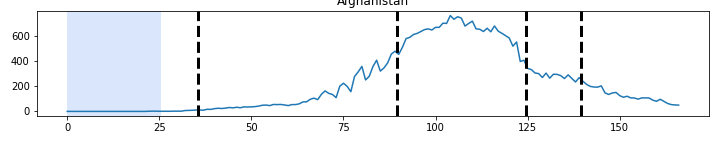
\includegraphics[width=0.9\textwidth]{_Afghanistan.png}
    \end{subfigure}
    \begin{subfigure}{\textwidth}
    	\centering
        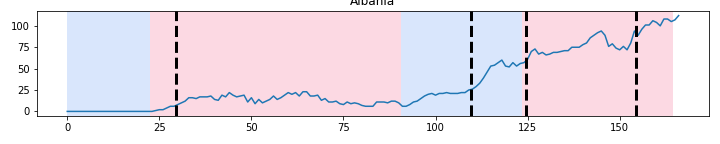
\includegraphics[width=0.9\textwidth]{_Albania.png}
    \end{subfigure}
   
    \begin{subfigure}{\textwidth}
    	\centering
        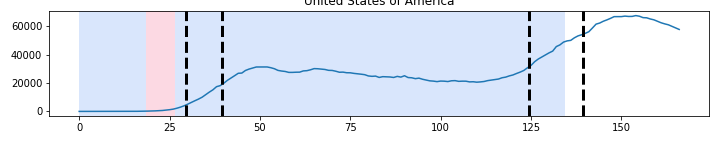
\includegraphics[width=0.9\textwidth]{_United States of America.png}
    \end{subfigure}
     \begin{subfigure}{\textwidth}
    	\centering
        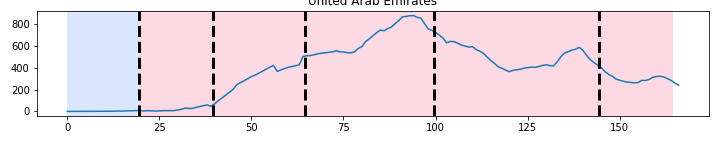
\includegraphics[width=0.9\textwidth]{_United Arab Emirates.png}
    \end{subfigure}
    \begin{subfigure}{\textwidth}
    	\centering
        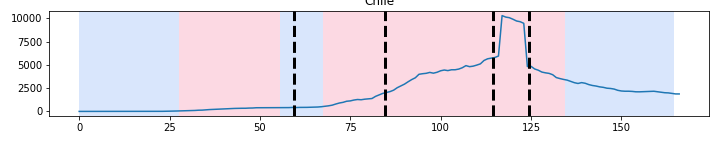
\includegraphics[width=0.9\textwidth]{_Chile.png}
    \end{subfigure}
    \begin{subfigure}{\textwidth}
    	\centering
        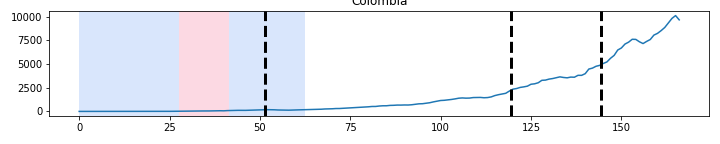
\includegraphics[width=0.9\textwidth]{_Colombia.png}
    \end{subfigure}
    \begin{subfigure}{\textwidth}
    	\centering
        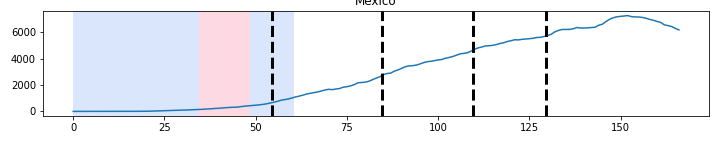
\includegraphics[width=0.9\textwidth]{_Mexico.png}
    \end{subfigure}
    \begin{subfigure}{\textwidth}
    	\centering
        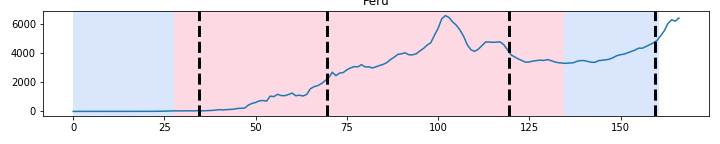
\includegraphics[width=0.9\textwidth]{_Peru.png}
    \end{subfigure}
  
    \caption{Change point detection.}
\label{fig:changepoint2}
\end{figure}





\end{document}
